\chapter{Representações da transformada de Fourier e diagramas de espectro}
Neste capítulo apresentaremos as representações da transformada de Fourier e introduziremos o conceito de diagramas de espectro.
\section{Forma trigonométrica}
A forma exponencial da transformada de Fourier de uma função $f(t)$ foi definida no capítulo \ref{trans_Fourier} e é dada por
\begin{equation}
F(w)=\mathcal{F}\{f(t)\}=\int_{-\infty}^\infty f(t)e^{-iwt}dt.
\end{equation}
Se $f(t)$ é uma função real, então podemos separar a parte real e imaginária da transformada de Fourier, conforme a seguir:
\begin{eqnarray*}
F(w)&=&\mathcal{F}\{f(t)\}=\int_{-\infty}^\infty f(t)e^{-iwt}dt\\
&=&\int_{-\infty}^\infty f(t)\left(\cos(wt)-i\sen(wt)\right)dt\\
&=&\int_{-\infty}^\infty f(t)\cos(wt)dt-i\int_{-\infty}^\infty f(t)\sen(wt) dt\\
&:=&A(w)-iB(w),
\end{eqnarray*}
onde
\begin{eqnarray*}
A(w)&=&\int_{-\infty}^\infty f(t)\cos(wt)dt\\
B(w)&=&\int_{-\infty}^\infty f(t)\sen(wt) dt
\end{eqnarray*}
Nesses termos, a função $f(t)$ pode ser escrita como:
\begin{eqnarray*}
f(t)&=&\frac{1}{2\pi}\int_{-\infty}^\infty F(w)e^{iwt}dw\\
&=&\frac{1}{2\pi}\int_{-\infty}^\infty \left(A(w)-i B(w)\right)\left(\cos(wt)+i\sen(wt)\right)dw\\
&=&\frac{1}{2\pi}\int_{-\infty}^\infty\left( A(w)\cos(wt)+ B(w)\sen(wt)\right)dw\\&+&\frac{i}{2\pi}\int_{-\infty}^\infty \left(A(w)\sen(wt)- B(w)\cos(wt)\right)dw
\end{eqnarray*}
Usando o fato que $A(w)$ é uma função par e $B(w)$ é uma função ímpar, temos:
\begin{eqnarray*}
f(t)&=&\frac{1}{2\pi}\int_{-\infty}^\infty\left(A(w)\cos(wt)+ B(w)\sen(wt)\right)dw\\
&=&\frac{1}{\pi}\int_{0}^\infty\left( A(w)\cos(wt)+ B(w)\sen(wt)\right)dw
\end{eqnarray*}
A tabela abaixo compara as formas trigonométrica e exponencial das séries e transformadas de Fourier
\begin{equation}
\begin{array}{|c|c|c|}
\hline &&\\
&\hbox{Forma exponencial}&\hbox{Forma trigonométrica}\\&&\\  \hline &&\\
\hbox{Série de Fourier}&\displaystyle f(t)=\sum_{n=-\infty}^\infty C_n e^{i w_n t} & \displaystyle  f(t)=\frac{a_0}{2}+\sum_{n=1}^\infty\left( a_n \cos(w_nt)+b_n\sen(w_nt)\right)   \\&&\\\hline &&\\
\hbox{Transformada de Fourier} &\displaystyle f(t)=\frac{1}{2\pi}\int_{-\infty}^\infty F(w)e^{iwt}dw &\displaystyle f(t)=\frac{1}{\pi}\int_{0}^\infty \left( A(w)\cos(wt)+ B(w)\sen(wt)\right)dw \\   &&\\\hline
\end{array}
\end{equation}
\begin{ex}{\label{ex_trans_rep_1}} Considere a função $f(t)=e^{-at}u(t)$ onde $a$ é uma constante positiva e $u(t)$ é a função Heaviside. A transformada de Fourier $F(w)$ de $f(t)$ foi calculada no exercício \ref{transf_exp_heav} da página \pageref{transf_exp_heav} e é dada por:
\begin{equation*}
F(w)=\frac{a}{a^2+w^2}-\frac{iw}{a^2+w^2}.
\end{equation*}
Usando representação trigonométrica da transformada de Fourier, temos:
\begin{eqnarray*}
f(t)=\frac{1}{\pi}\int_{0}^\infty\left( A(w)\cos(wt)+ B(w)\sen(wt)\right)dw,
\end{eqnarray*}
onde
\begin{eqnarray*}
A(w)&=&\frac{a}{a^2+w^2}\\
B(w)&=&\frac{w}{a^2+w^2}
\end{eqnarray*}
\end{ex}
\section{Diagramas de espectro}
Diagrama de espectro da transformada de Fourier é a representação gráfica da transformada de Fourier $F(w)$ associadas a uma função $f(t)$. Da mesma forma como o diagrama de espectro da série de Fourier se divide em amplitude e fase, o diagrama de espectro da transformada de Fourier se divide em magnitude e fase. Ou seja, o gráfico de $|F(w)|$ é a diagrama de magnitude e o gráfico de $\phi(w)$ é o diagrama de fase, onde
\begin{equation}
F(w)=|F(w)|e^{i\phi(w)},
\end{equation}
\begin{ex}No exemplo \ref{ex_Transf_1} da página \pageref{ex_Transf_1} calculamos a transformada de Fourier da função $f(t)=e^{-|t|}$:
\begin{equation}
F(w)=\frac{2}{w^2+1}.
\end{equation}
O gráfico da magnitude $|F(w)|$ é dado na figura \ref{diag_espec_trans_1}. Devido o fato de $F(w)$ ser real, a fase é uma função nula.
\begin{figure}[!ht]
\begin{center}
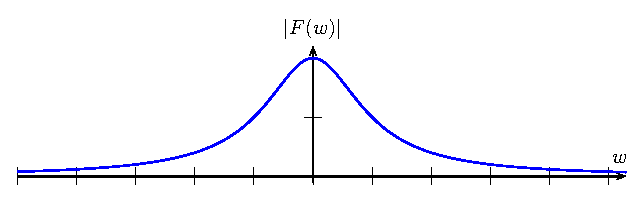
\includegraphics{cap_diagramas_espectro_transformada/pics/figura_1}\end{center}
\caption{\label{diag_espec_trans_1}}
\end{figure}
\end{ex}
\begin{ex} O exemplo \ref{ex_trans_rep_1} da página \pageref{ex_trans_rep_1} apresenta a transformada de Fourier da função $f(t)=e^{-at}u(t)$ onde $a$ é uma constante positiva e $u(t)$ é a função Heaviside: 
\begin{equation*}
F(w)=\frac{a}{a^2+w^2}-\frac{iw}{a^2+w^2}.
\end{equation*}
Observe que
\begin{eqnarray*}
|F(w)|&=&\sqrt{\left(\frac{a}{a^2+w^2}\right)^2+\left(\frac{w}{a^2+w^2}\right)^2}\\
&=&\sqrt{\frac{a^2+w^2}{\left(a^2+w^2\right)^2}}\\&=&\frac{1}{\sqrt{a^2+w^2}}
\end{eqnarray*}
e, como $a>0$, temos $\frac{a}{a^2+w^2}>0$. Portanto,
\begin{equation}
\phi(w)=\tan^{-1}\left(\frac{-\frac{w}{a^2+w^2}}{\frac{a}{a^2+w^2}}\right)=-\tan^{-1}\left(\frac{w}{a}\right).
\end{equation}
A figura \ref{diag_espec_trans_2} apresenta o diagrama de espectro de magnitude e fase da transformada $F(w)$ de $f(t)$ quando $a=1$.
\begin{figure}[!ht]
\begin{center}
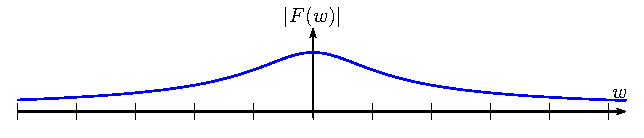
\includegraphics{cap_diagramas_espectro_transformada/pics/figura_2}
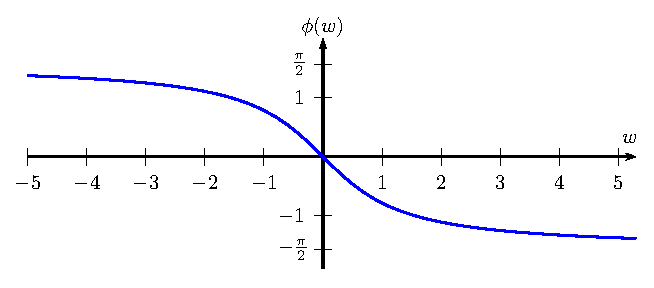
\includegraphics{cap_diagramas_espectro_transformada/pics/figura_3}\end{center}
\caption{\label{diag_espec_trans_2}}
\end{figure}
\end{ex}
\section{Exercícios}
\begin{Exercise}Mostre que a representação trigonométrica da transformada de Fourier $F(w)$ de uma função real $f(t)$ separa-a em parte ímpar e parte par. Isto é,
\begin{eqnarray*}
\frac{1}{\pi}\int_{0}^\infty A(w)\cos(wt)dw=\frac{f(t)+f(-t)}{2}
\end{eqnarray*}
e
\begin{eqnarray*}
\frac{1}{\pi}\int_{0}^\infty B(w)\sen(wt)dw=\frac{f(t)-f(-t)}{2}.
\end{eqnarray*}
\end{Exercise}
\begin{Exercise}Mostre que se $f(t)$ é real, $F(-w)=\overline{F(w)}$.
\end{Exercise}
\begin{Exercise}{\label{exer_te_t2}} Calcule a transformada de Fourier e trace o diagrama de espectro da função $f(t)=te^{-t^2}$. [Dica: Use integração por partes para transformar a integral dada numa integral tabelada].
\end{Exercise}
\begin{Answer}
\begin{eqnarray*}
F(w)=\int_{-\infty}^\infty te^{-t^2}e^{-iwt}dt&=&-2i\int_{0}^\infty te^{-t^2}\sen(wt)dt\\
&=&-2i\left[-\frac{e^{-t^2}}{2}\sen(wt) \right]_0^\infty+2i\int_{0}^\infty \left(-\frac{e^{-t^2}}{2}\right)w\cos(wt)dt\\
&=&-iw\int_{0}^\infty e^{-t^2}\cos(wt)dt\\
&=&-iw\frac{\sqrt{\pi}}{2}e^{-\frac{w^2}{4}}=|F(w)|e^{i\phi(w)}
\end{eqnarray*}
onde
\begin{eqnarray*}
|F(w)|=|w|\frac{\sqrt{\pi}}{2}e^{-\frac{w^2}{4}}\qquad\hbox{ e }\qquad \phi(w)&=&\left\{\begin{array}{ll}
-\frac{\pi}{2},&w>0,\\[.3cm]
\frac{\pi}{2},&w<0.
\end{array}\right.
\end{eqnarray*}
Veja o diagrama de espectro na figura abaixo.
\begin{center}
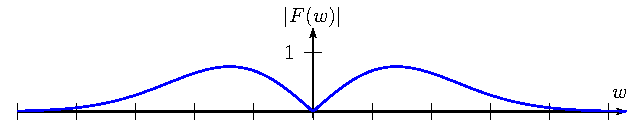
\includegraphics{cap_diagramas_espectro_transformada/pics/figura_4}
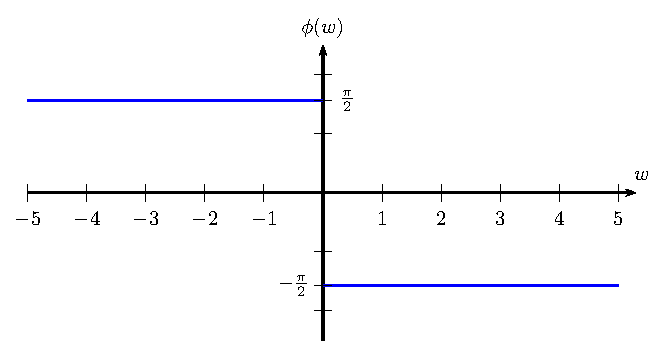
\includegraphics{cap_diagramas_espectro_transformada/pics/figura_5}\end{center}
\end{Answer}
